\chapter{Conceptual Evolution and Rationale}
\label{chap:Conceptual_Evolution_and_Rationale}
\textbf{Authors:} Luna Schaetzle

This chapter presents a comprehensive analysis of the conceptual and technical evolution of the project within the context of this Diploma Thesis. The investigation delineates the progression from an initial theoretical proposal, through intermediate developmental phases such as the Self-Sufficiency Raspberry Pi Project, to the formulation of the final design concept. Documenting this iterative transformation is critical to achieving a holistic understanding of the design process, as it underscores the dynamic interplay between feasibility constraints, scalability requirements, and alignment with overarching research objectives.

The discussion elucidates the key motivations, challenges, and pivotal decisions that shaped the project’s trajectory, with particular emphasis on evaluating technical and operational feasibility, ensuring scalable implementation frameworks, and maintaining coherence with core research goals. Furthermore, a critical examination of the technical obstacles encountered during prototyping and implementation phases is provided, highlighting how empirical insights informed subsequent refinements. By synthesizing these elements, this chapter not only chronicles the project’s developmental arc but also contextualizes the methodological rigor inherent in balancing theoretical aspirations with practical execution.

\section{Timeline and Milestones}

To provide a clear overview of the project's evolution, a timeline outlining the major milestones, decision points, and revisions is presented in the following chart.
\begin{figure}[H]
    \centering
    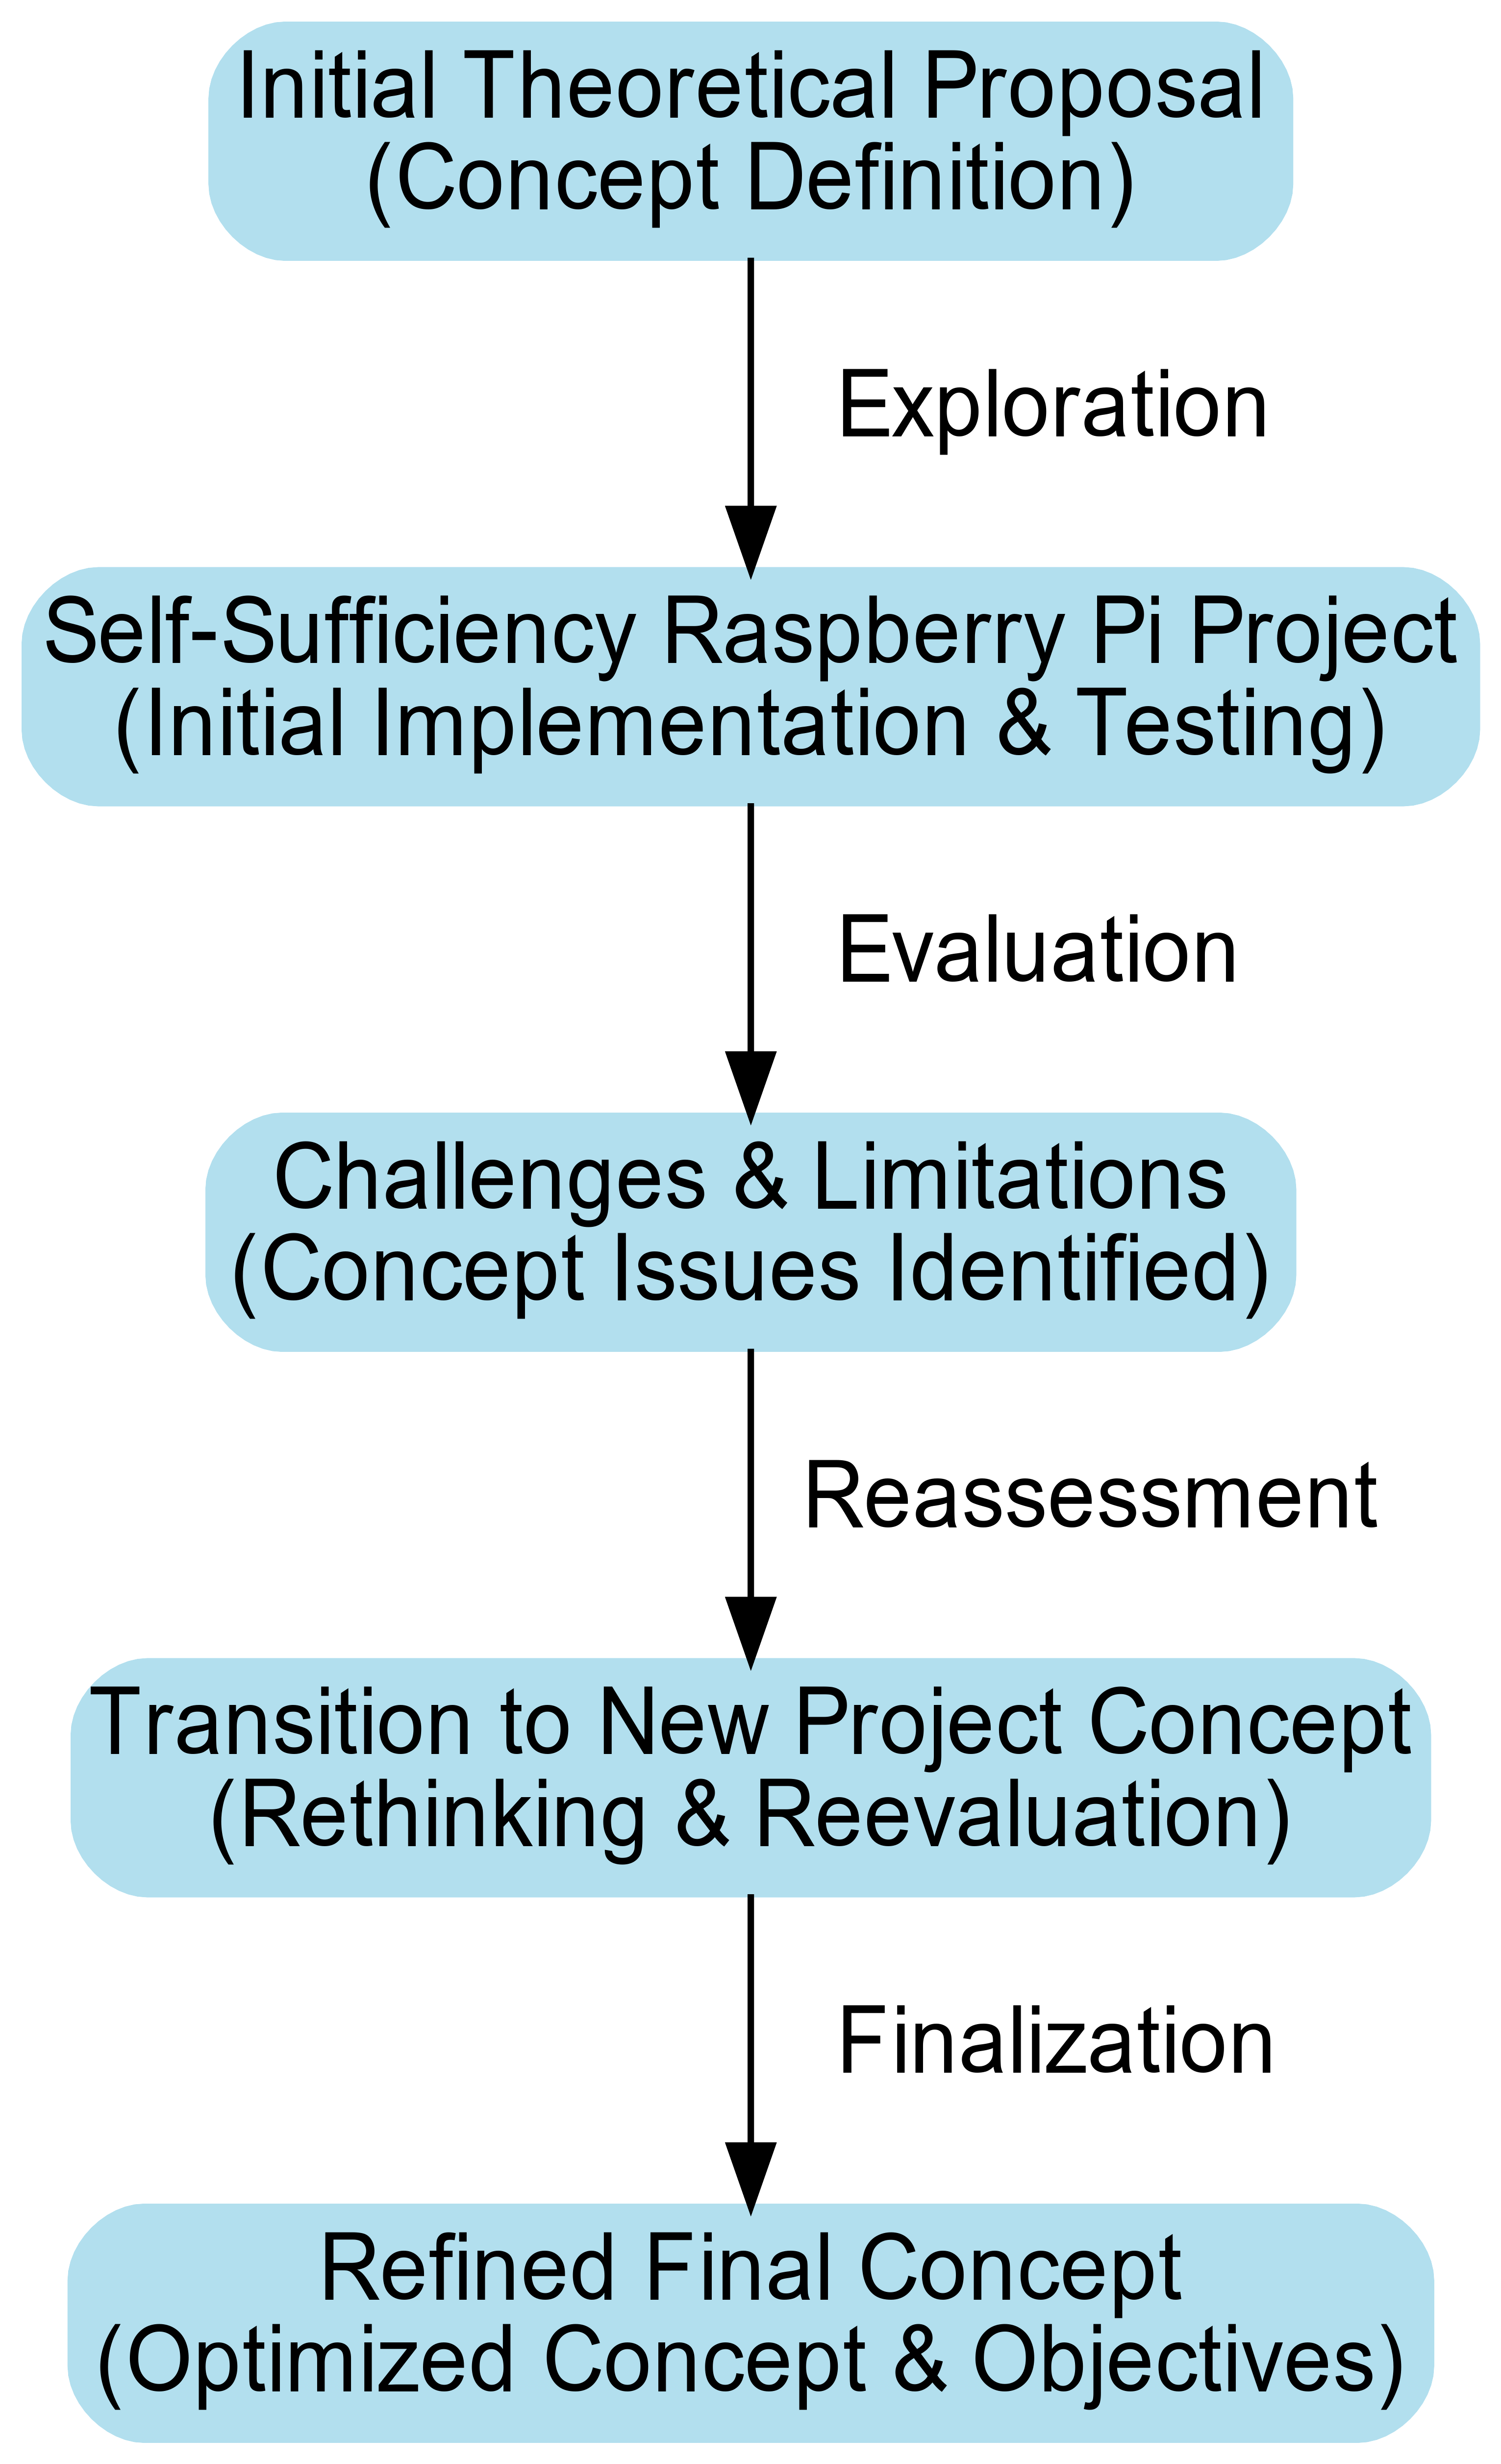
\includegraphics[width=0.4\textwidth]{figures/concept_change_flowchart.png}
    \caption{Gantt Chart of the Project Evolution}
    \label{fig:GanttChart}
\end{figure}

This timeline visually summarizes the progression of ideas and the key changes made over time, offering a concise reference to the project's developmental history.

\section{Initial Concept}

The initial concept for this Diploma Thesis was to explore various methodologies for leveraging Artificial Intelligence (AI) across diverse application domains. The primary objective was to develop a comprehensive framework for evaluating the performance of AI models in a range of tasks and use cases. This framework was intended to include both quantitative metrics and qualitative assessments, facilitated in part by the use of structured questionnaires to capture user experiences and application-specific requirements. However, early analysis revealed that the scope of this concept was overly broad. The project team quickly recognized that the lack of a focused research question, as well as the ambiguous integration of the various components, would make it challenging to implement the project within the available time and resources.

\section{The Self-Sufficiency Raspberry-PI project}

In response to these challenges, the project team refined its approach by narrowing the scope to a more tangible and achievable idea—the Self-Sufficiency Project. This project was designed around the development of a self-contained system based on a Raspberry Pi, capable of autonomously executing a variety of tasks. The core idea was to demonstrate a practical application of AI by minimizing reliance on external APIs and services, thereby increasing system robustness and independence. Additionally, the design emphasized portability, with the entire system housed in a compact enclosure to facilitate deployment in diverse environments. Figure~\ref{fig:SelfSufficiencyProject} illustrates the conceptual framework of the Self-Sufficiency Raspberry Pi Project.

\begin{figure}[H]
    \centering
    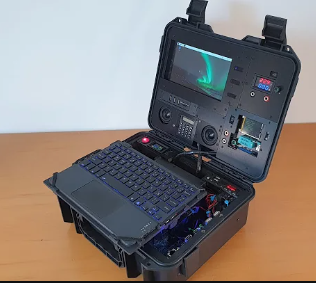
\includegraphics[width=0.5\textwidth]{figures/SAIPIA-concept-picture.png}
    \caption{Conceptual Illustration of the Self-Sufficiency Raspberry Pi Project}
    \label{fig:SelfSufficiencyProject}
\end{figure}

\cite{SAIPIA-Concept}

\section{Challenges and Limitations of the Self-Sufficiency Raspberry-PI Project}

During the development of the Self-Sufficiency Project, several significant challenges and limitations emerged that prompted a critical reassessment of the project’s direction. These challenges included:
\begin{itemize}
    \item \textbf{Complexity of Implementation:} The integration of heterogeneous AI models with multiple hardware components introduced considerable technical difficulties, necessitating extensive iterative development and rigorous testing.
    \item \textbf{Scalability Constraints:} The self-sufficiency paradigm, while beneficial for system independence, inherently restricted scalability and interoperability with external systems, thereby limiting future expansion.
    \item \textbf{Resource Limitations:} The ambitious scope of the project, combined with constrained time and technical expertise, rendered the initial plan impractical.
    \item \textbf{Ambiguity in Objectives:} The absence of clearly defined, measurable goals complicated the assessment of progress and the determination of success criteria.
    \item \textbf{Integration Challenges:} The complexity of harmonizing various AI models, hardware interfaces, and supporting software systems proved to be more formidable than initially anticipated.
    \item \textbf{Time Constraints:} Preliminary evaluations indicated that the project’s timeline was insufficient to address the technical and logistical challenges identified.
\end{itemize}

In light of these challenges, the project team concluded that a more narrowly defined and feasible approach was necessary. Consequently, the focus shifted towards a new concept that emphasizes AI applications and their specific use cases.

\section{Transition to the Current Project Concept}

After reevaluating the limitations of the initial approaches, the project team restructured the initiative into a more focused framework, subdividing it into three distinct components. This revised approach not only addresses the previously identified constraints but also aligns more closely with the overarching research objectives. The current project concept is organized into the following three components:

\subsection{AI for Education}

This component explores the integration of AI technologies within educational settings. The primary goal is to develop an AI-powered web application that facilitates interactive and personalized learning experiences, particularly for IT students. By leveraging adaptive learning algorithms, the system aims to enhance comprehension and engagement, thereby contributing to more effective educational practices.

\subsection{AI Integration in Software Development}

Focusing on the software development domain, this component investigates how AI can assist developers in writing and debugging code. The objective is to develop an AI model that integrates seamlessly into the development workflow, for example, via a Visual Studio Code extension. This extension is designed to provide real-time code analysis, suggestions, and bug detection, ultimately improving code quality and development efficiency.


\section{Overcoming Challenges in the Current Project Concept}

The evolution of any project is accompanied by a series of challenges. In transitioning to the current project concept, the team identified and addressed several critical obstacles to ensure a robust and effective implementation of the new framework.

\subsection{Challenges}

The primary challenges encountered during this transition included:

\begin{itemize}
    \item \textbf{Technical Complexity:} Integrating advanced AI models with diverse platforms—such as web applications and code editors required a deep understanding of multiple technologies and frameworks.
    \item \textbf{Resource Limitations:} The expansive scope of the project necessitated a judicious allocation of time, technical expertise, and hardware resources.
    \item \textbf{Scalability Issues:} Balancing the goal of system independence with the need for scalability and interoperability posed a significant challenge.
    \item \textbf{Temporal Constraints:} The limited project timeline imposed restrictions on the depth and breadth of research and development activities.
    \item \textbf{Integration Complexity:} Harmonizing the heterogeneous components of the project—including AI models, hardware interfaces, and software systems—proved more intricate than initially anticipated.
    \item \textbf{Ambiguity in Evaluation Criteria:} The absence of clearly definable, quantifiable success metrics complicated the objective assessment of project progress and outcomes.
    \item \textbf{Server Resource Limitations:} Particularly within the AI for Education component, limitations in server capacity emerged as a significant impediment to achieving desired scalability.
\end{itemize}

\subsection{Solutions}

In response to these challenges, the project team adopted a series of strategic measures:

\begin{itemize}
    \item \textbf{Modularization:} Dividing the project into three distinct components allowed for a more focused development approach, effectively managing complexity and scalability concerns.
    \item \textbf{Scope Refinement:} By narrowing the project’s scope, the team could allocate resources more efficiently, thereby establishing a realistic timeline and achievable milestones.
    \item \textbf{Iterative Development:} Implementing an iterative development methodology enabled the incremental resolution of technical challenges, leading to a more robust and scalable final implementation.
    \item \textbf{Optimization of Server Resources:} Specific efforts were made to streamline the AI for Education component, thereby reducing server resource consumption and mitigating scalability issues.
    \item \textbf{Establishment of Clear Evaluation Metrics:} The development and adoption of explicit, measurable evaluation criteria for each project component facilitated systematic progress tracking and performance assessment.
    \item \textbf{Utilization of AI for Process Optimization:} Leveraging AI technologies to automate routine tasks and optimize overall system performance further enhanced efficiency and scalability.
\end{itemize}

\section{Insights and Lessons Learned}

Throughout the project’s evolution, several key insights were gained, which have significantly informed the current project concept and its implementation strategy. These insights include:

\begin{itemize}
    \item \textbf{Adaptive Planning:} The capacity to adapt and refine project parameters in response to emerging challenges is critical for successful project execution.
    \item \textbf{Incremental Development:} An iterative development approach facilitates steady progress and enables the timely resolution of technical issues, contributing to continuous improvement of the project design.
    \item \textbf{Strategic Resource Allocation:} Effective management of available resources—time, expertise, and hardware—is essential for mitigating complexity and ensuring the project’s successful completion.
    \item \textbf{Balancing Independence and Scalability:} Striking the right balance between system autonomy and scalability is paramount for ensuring long-term viability and facilitating future integrations.
    \item \textbf{Clear Metrics for Evaluation:} Establishing definitive, quantifiable success metrics is vital for tracking progress, objectively assessing outcomes, and guiding subsequent development efforts.
    \item \textbf{Leveraging AI for Optimization:} The strategic use of AI to automate processes and optimize system performance can markedly enhance overall efficiency and scalability.
    \item \textbf{Importance of Targeted Optimization Strategies:} Focused measures—such as reducing server resource usage and refining AI model implementations—are crucial for addressing scalability concerns and boosting system performance.
\end{itemize}

\section{Conclusion}

%In summary, this chapter has provided a comprehensive overview of the project's conceptual evolution—from an initially broad theoretical framework to a refined and focused approach. The early phases, characterized by the exploration of diverse methodologies for leveraging AI, gradually evolved through the practical implementation of the Self-Sufficiency Raspberry Pi Project. This progression illuminated significant challenges, including technical complexities, resource limitations, and scalability issues, which ultimately necessitated a critical reassessment of the project’s scope.

The transition to the current project concept was driven by a deliberate process of modularization, scope refinement, 
and iterative development. By segmenting the initiative into three distinct components AI for Education and AI Integration in Software Development 
the project team was able to align the research objectives with practical constraints and emerging technological opportunities. 
The strategic measures implemented to overcome obstacles, along with the insights and lessons learned throughout this evolution, 
have established a robust foundation for future development.

Overall, the iterative nature of this process underscores the importance of adaptive planning, 
igorous evaluation, and targeted optimization strategies in the successful execution of complex projects. 
The refined concept not only addresses the initial challenges but also sets a clear pathway for the subsequent phases of the Diploma Thesis, 
paving the way for a detailed exploration of each component in the chapters that follow.

